\chapter{Architectures}



\graphicspath{{../../year1/image-processing-and-computer-vision/module2/}}


\section{Inception-v1 (GoogLeNet)\protect\footnote{Excerpt from \href{https://raw.githubusercontent.com/NotXia/unibo-ai-notes/pdfs/year1/image-processing-and-computer-vision/module2/ipcv2.pdf}{IPCV2}}}
\marginnote{Inception-v1 (GoogLeNet)}

Network that aims to optimize computing resources (i.e., small amount of parameters and FLOPs).

\begin{description}
    \item[Stem layers]
        Down-sample the image from a shape of 224 to 28.
        As in ZFNet, multiple layers are used (5) and the largest convolution is of shape $7 \times 7$ with stride $2$.

    \item[Inception module] \marginnote{Inception module}
        Main component of Inception-v1 that computes multiple convolutions on the input.

        Given the input activation, the output is the concatenation of:
        \begin{itemize}
            \item A $1 \times 1$ (stride $1$) and a $5 \times 5$ (stride $1$, padding $2$) convolution.
            \item A $1 \times 1$ (stride $1$) and a $3 \times 3$ (stride $1$ and padding $1$) convolution.
            \item A $1 \times 1$ (stride $1$ and padding $0$) convolution.
            \item A $1 \times 1$ (stride $1$) convolution and a $3 \times 3$ (stride $1$ and padding $1$) max-pooling.
        \end{itemize} 

        \begin{figure}[H]
            \centering
            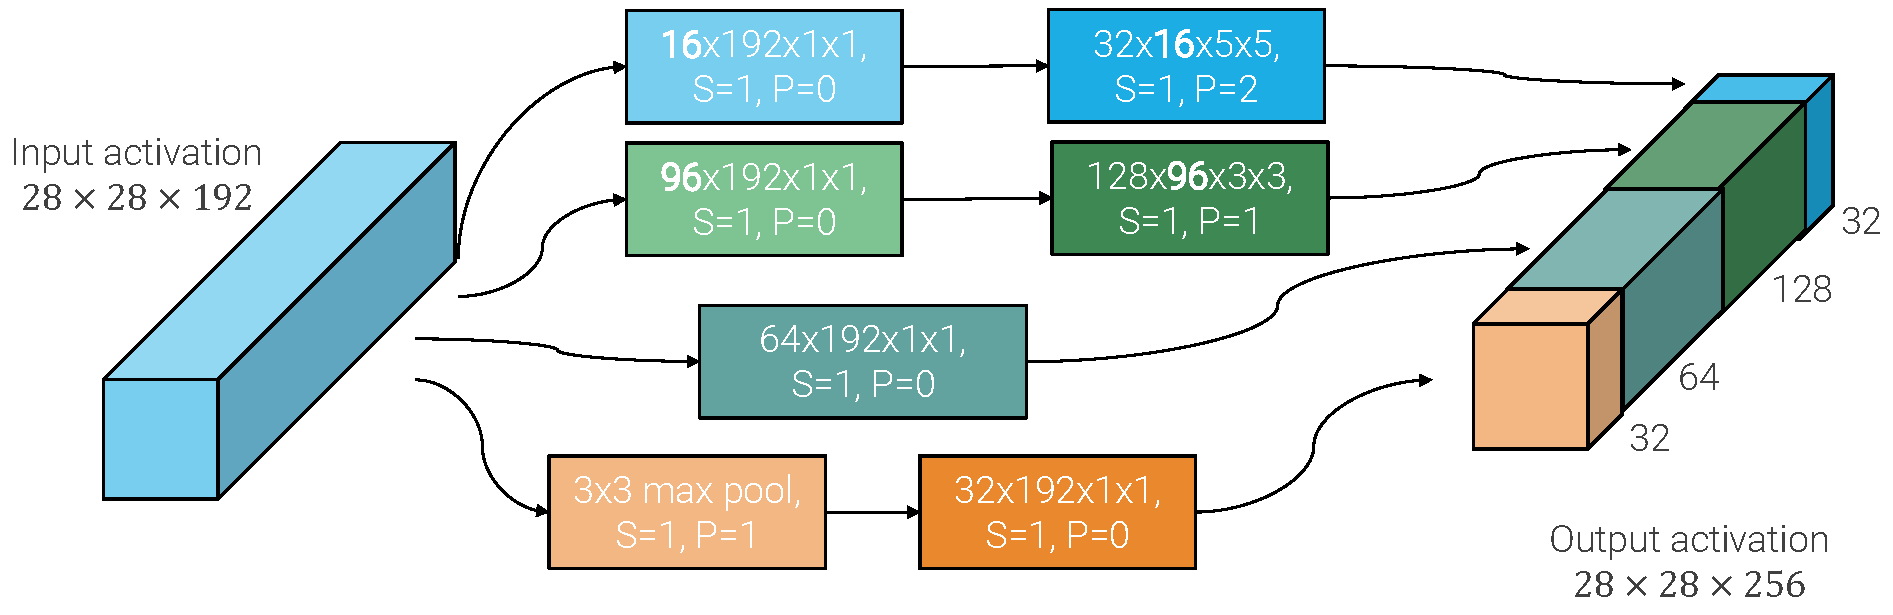
\includegraphics[width=0.6\linewidth]{./img/_actual_inception.pdf}
            \caption{Inception module on the output of the stem layers}
        \end{figure}

        \begin{remark}
            The multiple convolutions of an inception module can be seen as decision components.
        \end{remark}

    \item[Auxiliary \texttt{softmax}]
        Intermediate \texttt{softmax}s are used to ensure that hidden features are good enough.
        They also act as regularizers. During inference, they are discarded.

    \item[Global average pooling classifier] \marginnote{Global average pooling classifier}
        Instead of flattening between the convolutional and fully connected layers, 
        global average pooling is used to reduce the number of parameters.
\end{description}

\begin{figure}[H]
    \centering
    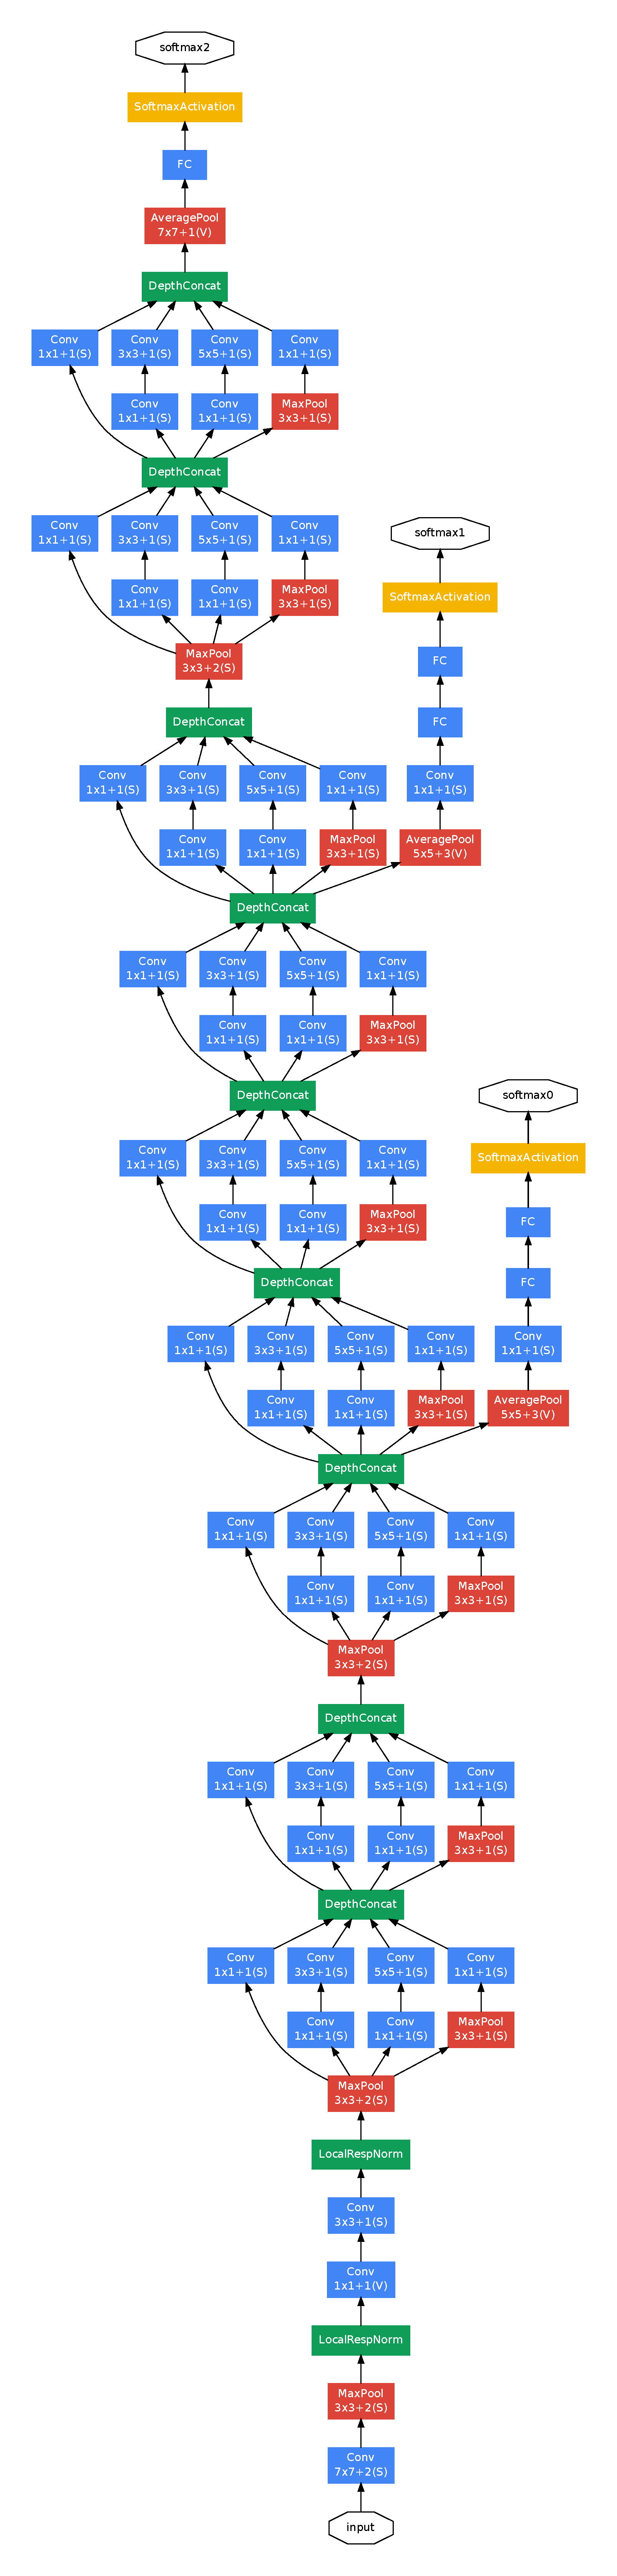
\includegraphics[angle=-90, width=0.7\linewidth]{./img/_inception_v1.pdf}
    \caption{Architecture of Inception-v1}
\end{figure}



\section{Residual networks\protect\footnote{Excerpt from \href{https://raw.githubusercontent.com/NotXia/unibo-ai-notes/pdfs/year1/image-processing-and-computer-vision/module2/ipcv2.pdf}{IPCV2}}}

\begin{description}
    \item[Standard residual block] \marginnote{Standard residual block}
        Block that allows to easily learn the identity function through a skip connection.
        The output of a residual block with input $x$ and a series of convolutional layers $F$ is:
        \[ F(x; \matr{\theta}) + x \]

        \begin{minipage}{0.75\linewidth}
            \begin{description}
                \item[Skip connection] \marginnote{Skip connection}
                    Connection that skips a certain number of layers (e.g. 2 convolutional blocks).
            \end{description}
    
            \begin{remark}
                Training starts with small weights so that the network starts as the identity function. Updates can be seen as perturbations of the identity function.
            \end{remark}
    
            \begin{remark}
                Batch normalization is heavily used.
            \end{remark}
        \end{minipage}
        \begin{minipage}{0.2\linewidth}
            \centering
            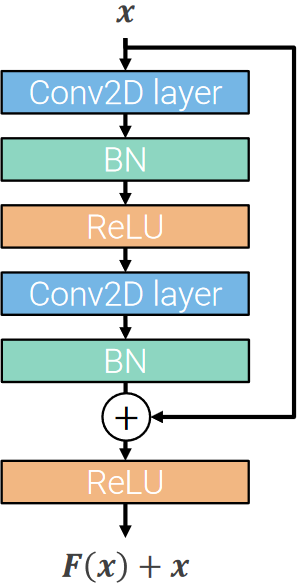
\includegraphics[width=0.8\linewidth]{./img/skip_conn.png}
        \end{minipage}
        
        \begin{remark}
            Skip connections are applied before the activation function (ReLU) as otherwise it would be summed to all positive values making the perturbation of the identity function less effective.
        \end{remark}
\end{description}


\subsection{ResNet}
\marginnote{ResNet-18}

VGG-inspired network with residual blocks.
It has the following properties:\\
\begin{minipage}{0.48\linewidth}
    \begin{itemize}
        \item A stage is composed of residual blocks.
        \item A residual block is composed of two $3 \times 3$ convolutions followed by batch normalization.
        \item The first residual block of each stage halves the spatial dimension and doubles the number of channels (there is no pooling).
    \end{itemize}
\end{minipage}
\hfill
\begin{minipage}{0.45\linewidth}
    \begin{figure}[H]
        \centering
        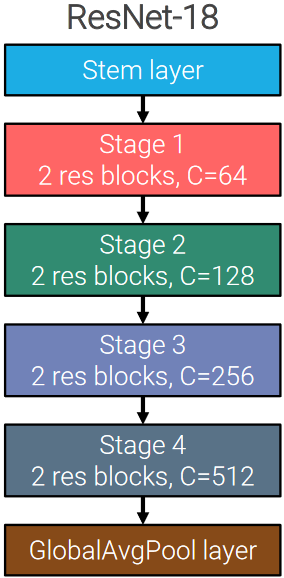
\includegraphics[width=0.35\linewidth]{./img/resnet_18.png}
        \caption{Architecture of ResNet-18}
    \end{figure}
\end{minipage}


\begin{description}
    \item[Bottleneck residual network] \marginnote{Bottleneck residual network}
        Variant of residual blocks that uses more layers with approximately the same number of parameters and FLOPs of the standard residual block.
        Instead of using two $3 \times 3$ convolutions, bottleneck residual network has the following structure:
        \begin{itemize}
            \item $1 \times 1$ convolution to compress the channels of the input by an order of $4$ (and the spatial dimension by $2$ if it is the first block of a stage, as in normal ResNet).
            \item $3 \times 3$ convolution.
            \item $1 \times 1$ convolution to match the shape of the skip connection.
        \end{itemize}

        \begin{figure}[H]
            \centering
            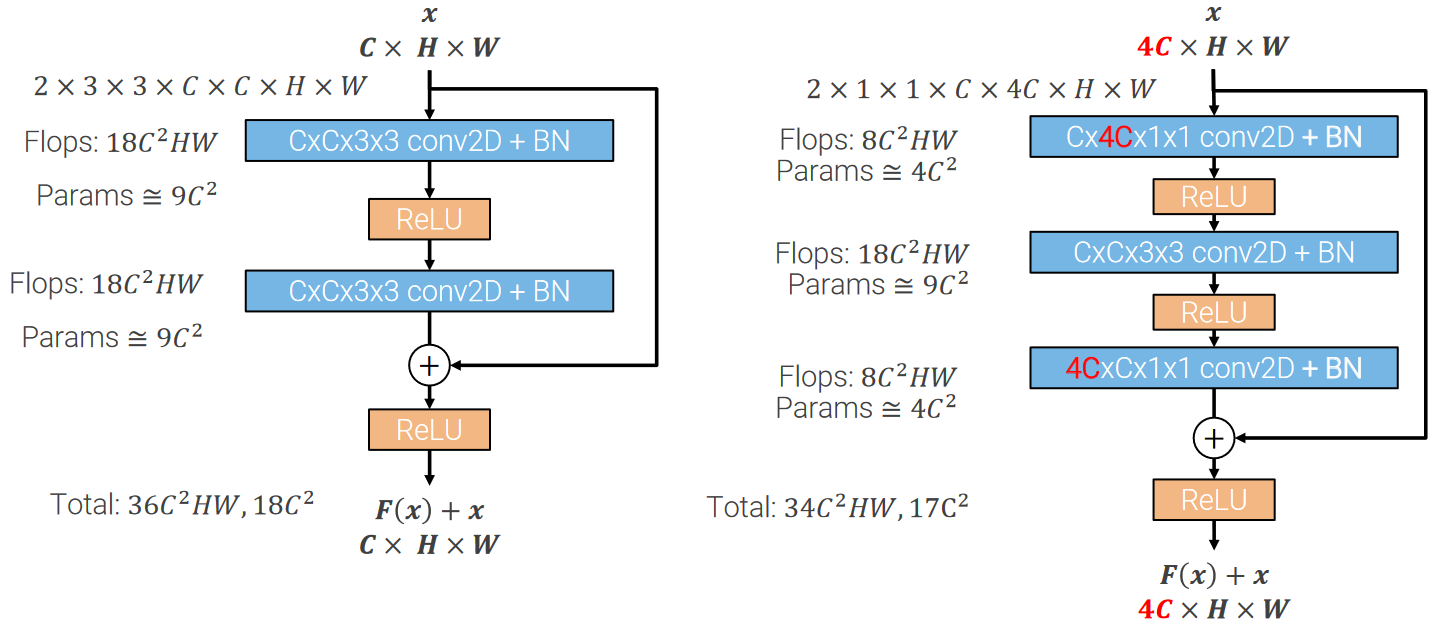
\includegraphics[width=0.8\linewidth]{./img/bottleneck_block.png}
            \caption{Standard residual block (left) and bottleneck block (right)}
        \end{figure}
\end{description}


\subsection{Inception-ResNet-v4}

Network with bottleneck-block-inspired inception modules.

\begin{descriptionlist}
    \item[Inception-ResNet-A] \marginnote{Inception-ResNet-A}
        Three $1 \times 1$ convolutions are used to compress the input channels. Each of them leads to a different path:
        \begin{itemize}
            \item Directly to the final concatenation.
            \item To a $3 \times 3$ convolution.
            \item To two $3 \times 3$ convolutions (i.e. a factorized $5 \times 5$ convolution). 
        \end{itemize}
        The final concatenation is passed through a $1 \times 1$ convolution to match the skip connection shape.

    \item[Inception-ResNet-B] \marginnote{Inception-ResNet-B}
        Three $1 \times 1$ convolutions are used to compress the input channels. Each of them leads to:
        \begin{itemize}
            \item Directly to the final concatenation.
            \item A $1 \times 7$ and $7 \times 1$ convolutions (i.e. a factorized $7 \times 7$ convolution). 
        \end{itemize}
        The final concatenation is passed through a $1 \times 1$ convolution to match the skip connection shape.
\end{descriptionlist}

\begin{figure}[H]
    \centering
    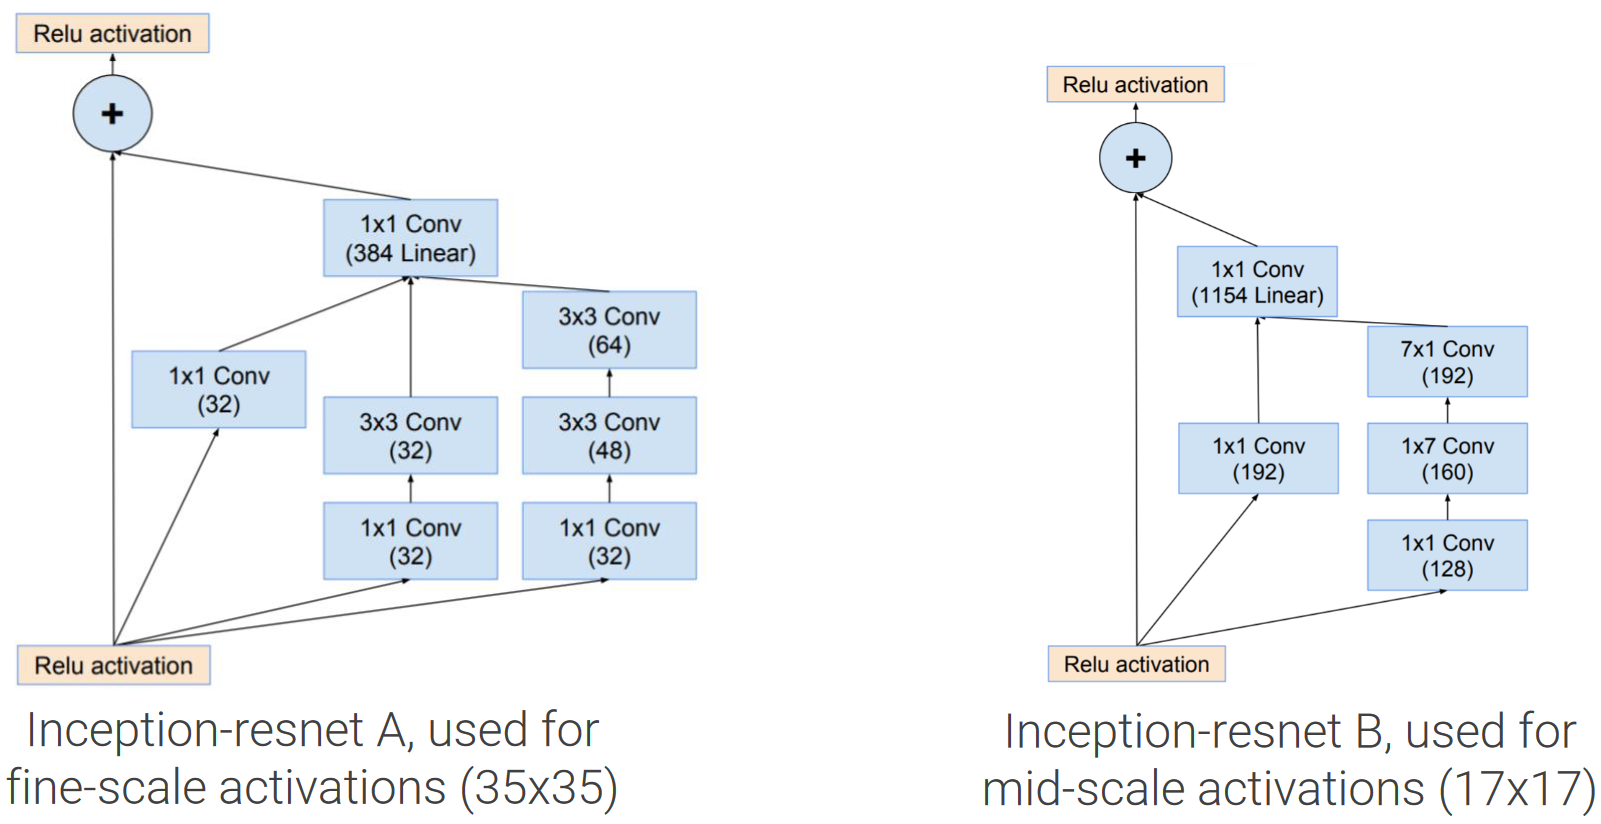
\includegraphics[width=0.5\linewidth]{./img/inception_resnet.png}
\end{figure}


\graphicspath{}



\section{ResNeXt}

\begin{remark}
    Inception and Inception-ResNet modules are multi-branch architectures and can be interpreted as a split-transform-merge paradigm. Moreover, their architectures have been specifically ``hand" designed.
\end{remark}

\begin{description}
    \item[Grouped convolution] \marginnote{Grouped convolution}
        Given:
        \begin{itemize}
            \item The input activation of shape $C_\text{in} \times W_\text{in} \times H_\text{in}$,\item The desired number of output channels $C_\text{out}$,
            \item The number of groups $G$,
        \end{itemize} 
        a grouped convolution splits the input into $G$ chunks of $\frac{C_\text{in}}{G}$ channels and processes each with a dedicated set of kernels of shape $\frac{C_\text{out}}{G} \times \frac{C_\text{in}}{G} \times W_K \times H_K$. The output activation is obtained by stacking the outputs of each group.

        \begin{figure}[H]
            \centering
            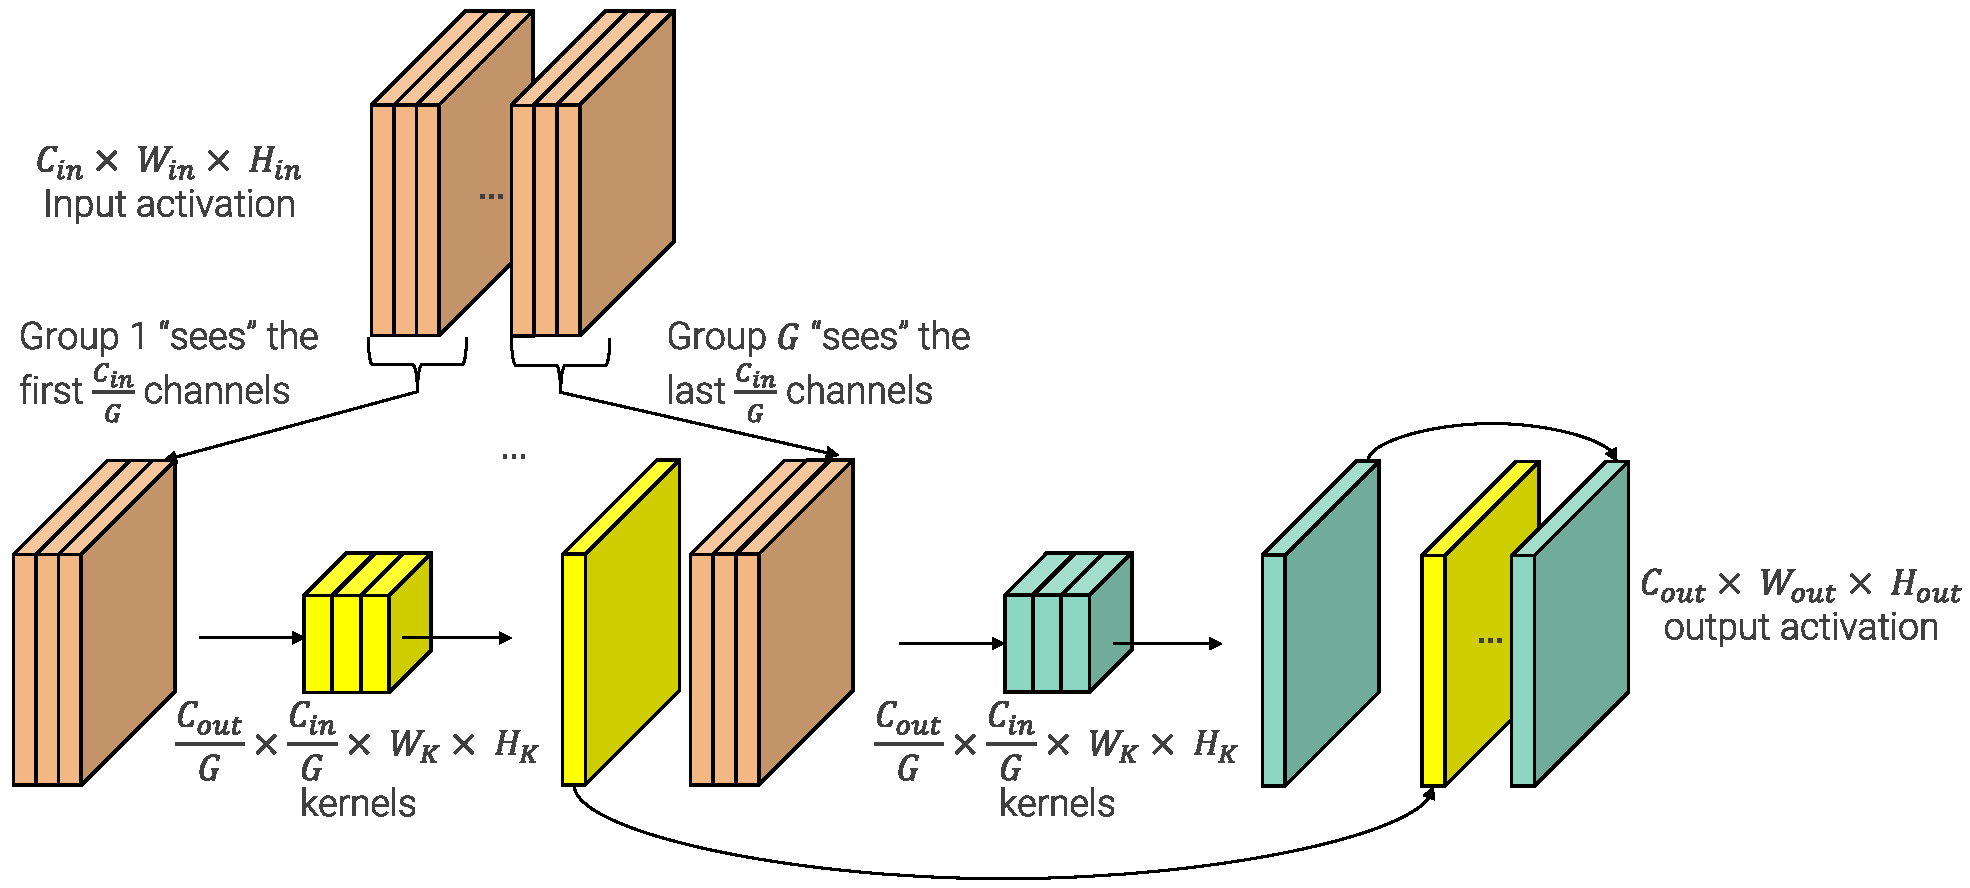
\includegraphics[width=0.7\linewidth]{./img/_grouped_conv.pdf}
        \end{figure}

        By processing the input in smaller chunks, there are the following gains:
        \begin{itemize}
            \item The number of parameters is $G$ times less.
            \item The number of FLOPs is $G$ times less.
        \end{itemize}

        \begin{remark}
            Grouped convolutions are trivially less expressive than convolving on the full input activation. However, as convolutions are expected to build a hierarchy of features, it is reasonable to process the input in chunks as, probably, not all of it is needed.
        \end{remark}
\end{description}

\begin{description}
    \item[ResNetXt block] \marginnote{ResNetXt block}
        Given the number of branches $G$ and the number of intermediate channels $d$, a ResNeXt block decomposes a bottleneck residual block into $G$ parallel branches that are summed out at the end.
        \begin{figure}[H]
            \centering
            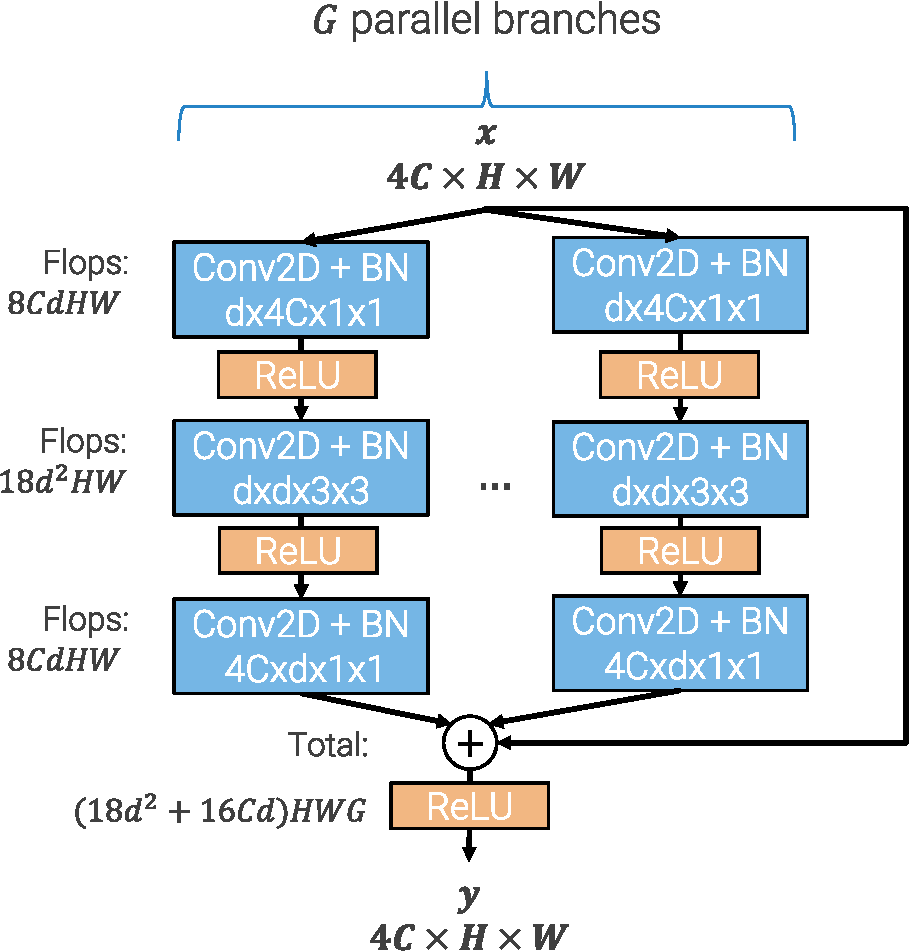
\includegraphics[width=0.35\linewidth]{./img/_resnext_block.pdf}
        \end{figure}

        \begin{remark}
            The branching in a ResNeXt block should not be confused with grouped convolutions.
        \end{remark}

        \begin{remark}
            Parametrizing $G$ and $d$ allows obtaining configurations that are FLOP-wise comparable with the original ResNet by fixing $G$ and solving a second-order equation over $d$.
        \end{remark}

        \begin{description}
            \item[Equivalent formulation]
                Given an input activation $\vec{x}$ of shape $4C \times H \times W$, each layer of the ResNeXt block can be reformulated as follows:
                \begin{descriptionlist}
                    \item[Second $1 \times 1$ convolution] 
                        Without loss of generality, consider a ResNeXt block with $G=2$ branches.

                        The output $\vec{y}_k$ at each channel $k=1, \dots, 4C$ is obtained as:
                        \[ \vec{y}_k = \vec{y}_k^{(1)} + \vec{y}_k^{(2)} + \vec{x}_k \]
                        where the output $\vec{y}_k^{(b)}$ of a branch $b$ is computed as:
                        \[
                            \begin{split}
                                \vec{y}_k^{(b)}(j, i) &= \left[ \vec{w}^{(b)} * \vec{a}^{(b)} \right]_k(j, i) \\
                                &= \vec{w}^{(b)}_k \cdot \vec{a}^{(b)}(j, i) \\
                                &= \vec{w}^{(b)}_k(1) \vec{a}^{(b)}(j, i, 1) + \dots + \vec{w}^{(b)}_k(d) \vec{a}^{(b)}(j, i, d)
                            \end{split}
                        \]
                        where:
                        \begin{itemize}
                            \item $*$ represents a convolution,
                            \item $\vec{a}^{(b)}$ is the input activation with $d$ channels from the previous layer.
                            \item $\vec{w}^{(b)}$ is the convolutional kernel. $\vec{w}^{(b)}_k \in \mathbb{R}^{d}$ is the kernel used to obtain the $k$-th output channel.
                        \end{itemize}

                        By putting everything together:
                        \[
                            \begin{split}
                                \vec{y}_k(j, i) &= \vec{w}^{(1)}_k \cdot \vec{a}^{(1)}(j, i) + \vec{w}^{(2)}_k \cdot \vec{a}^{(2)}(j, i) + \vec{x}_k \\
                                &= 
                                \underbrace{\left[ \vec{w}^{(1)}_k \vec{w}^{(2)}_k \right]}_{\hspace{1cm}\mathllap{\parbox{4cm}{\scriptsize by stacking, this is a $1\times1$ convolution with $2d$ channels}}}
                                \cdot 
                                \underbrace{\left[ \vec{a}^{(1)}(j, i) \vec{a}^{(2)}(j, i) \right] }_{\hspace{-1cm}\mathrlap{\parbox{4cm}{\scriptsize by stacking depth-wise, this is an activation with $2d$ channels}}}
                                +\, \vec{x}_k
                            \end{split}
                        \]
                        Therefore, the last ResNeXt layer with $G$ branches is equivalent to a single convolution with $Gd$ input channels that processes the concatenation of the activations of the previous layer.

                        \begin{figure}[H]
                            \centering
                            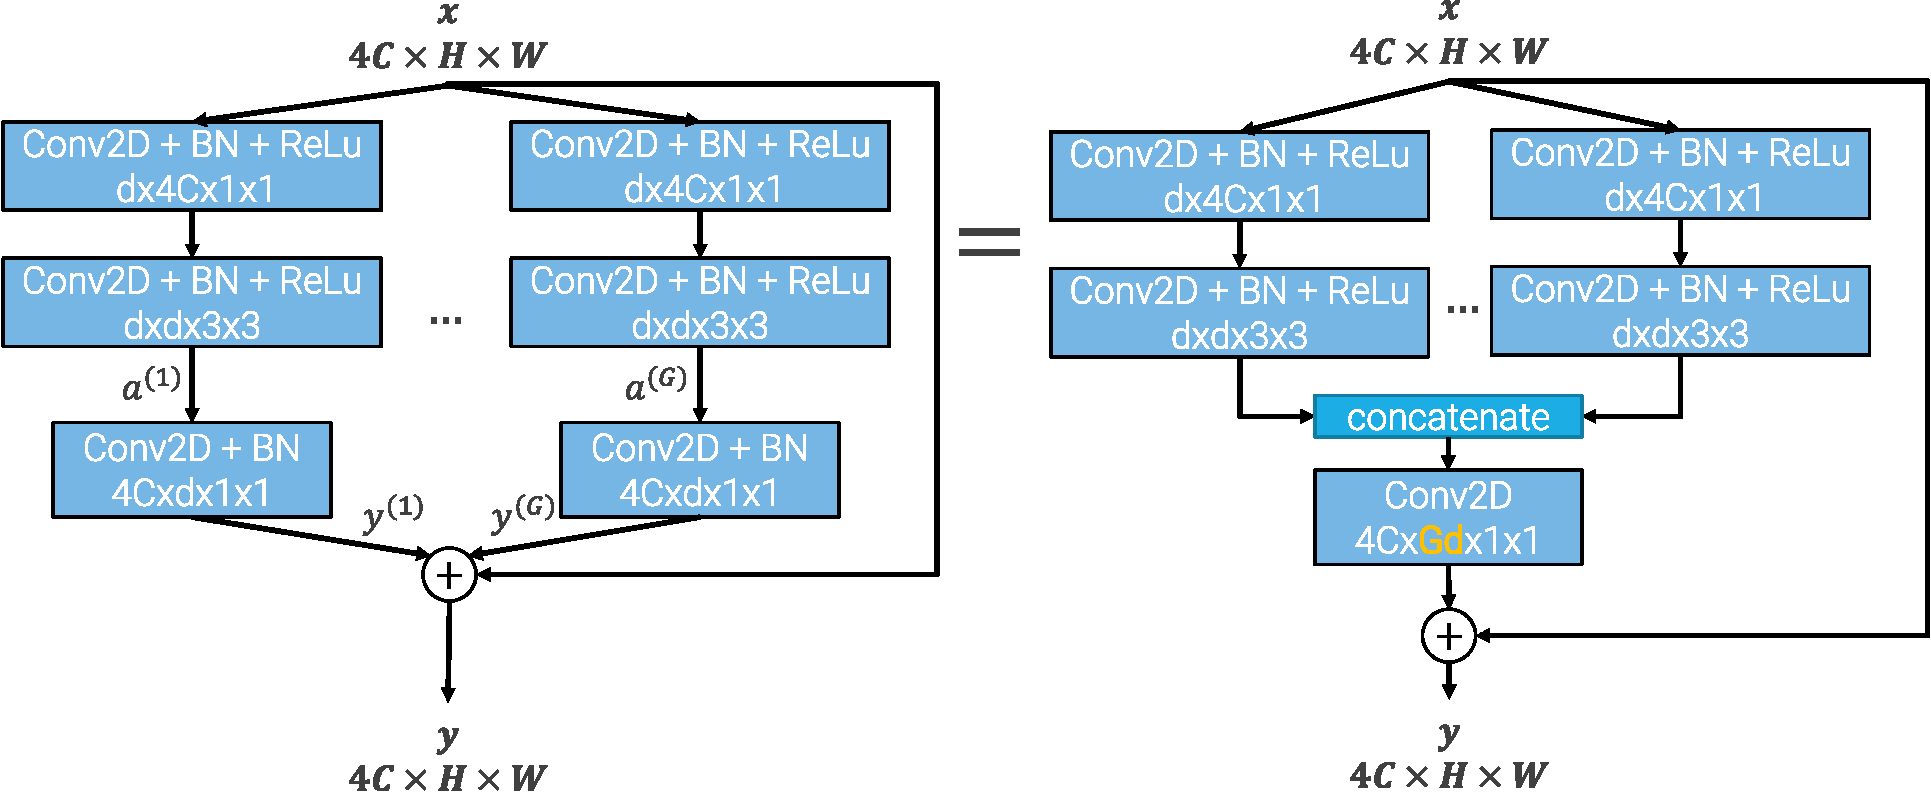
\includegraphics[width=0.8\linewidth]{./img/_resnext_to_resnet_l3.pdf}
                        \end{figure}

                    \item[First $1 \times 1$ convolution] 
                        The $G$ $1 \times 1$ convolutions at the first layer of ResNeXt all process the same input $\vec{x}$. Trivially, this can also be represented using a single $1 \times 1$ convolution with $G$ times more output channels that can be split afterwards.

                        \begin{figure}[H]
                            \centering
                            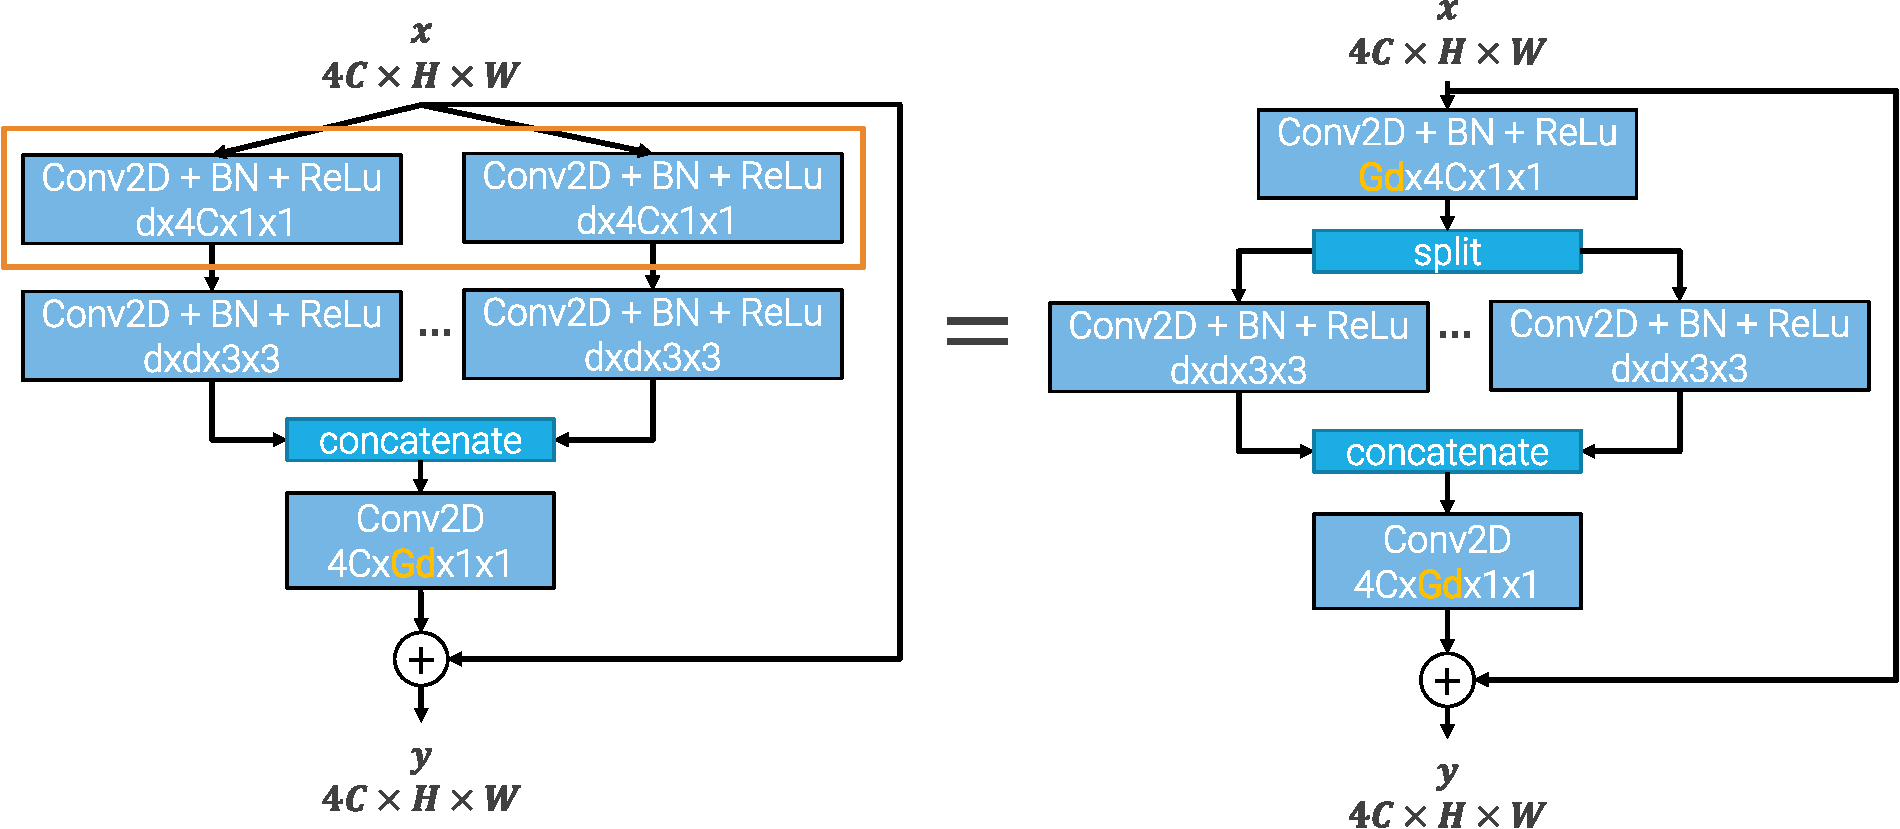
\includegraphics[width=0.8\linewidth]{./img/_resnext_to_resnet_l1.pdf}
                        \end{figure}

                    \item[$3 \times 3$ convolution] 
                        By putting together the previous two equivalences, the middle layer has the same definition of a grouped convolution with $G$ groups. Therefore, it can be seen as a single grouped convolution with $G$ groups and $Gd$ input and output channels.

                        \begin{figure}[H]
                            \centering
                            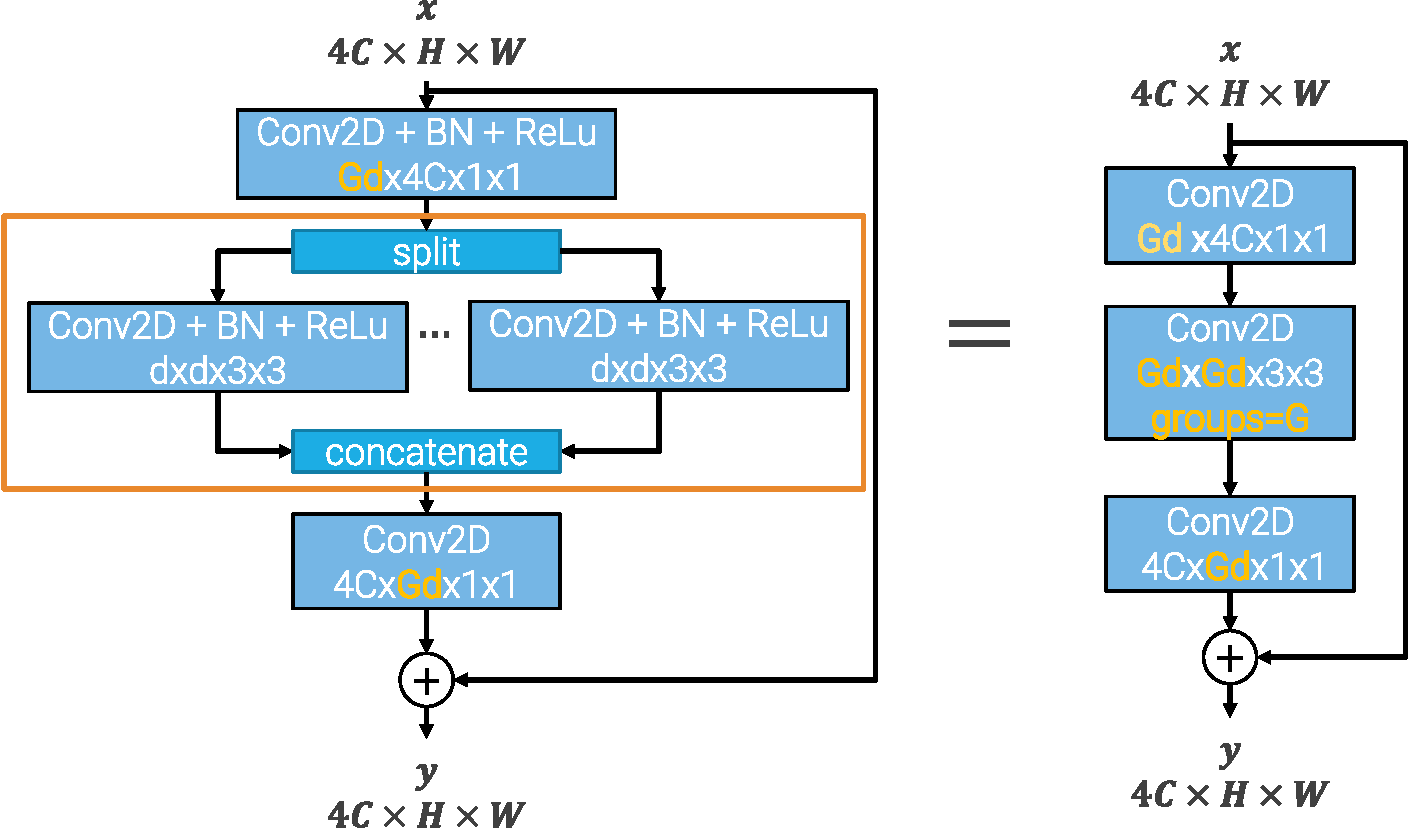
\includegraphics[width=0.6\linewidth]{./img/_resnext_to_resnet_l2.pdf}
                        \end{figure}
                \end{descriptionlist}

            \begin{remark}
                Therefore, a ResNeXt block is similar to a bottleneck block.
            \end{remark}
        \end{description}
\end{description}

\begin{remark}
    It has been empirically seen that, with the same FLOPs, it is better to have more groups (i.e., wider activations).
\end{remark}



\section{Squeeze-and-excitation network (SENet)}

\begin{description}
    \item[Squeeze-and-excitation module] \marginnote{Squeeze-and-excitation module}
        Block that weighs the channels of the input activation.
        Given the $c$-th channel of the input activation $\vec{x}_c$, the output $\tilde{\vec{x}}_c$ is computed as:
        \[ \tilde{\vec{x}}_c = s_c \vec{x}_c \]
        where $s_c \in [0, 1]$ is the scaling factor.

        The two operations of a squeeze-and-excitation block are:
        \begin{descriptionlist}
            \item[Squeeze]
                Global average pooling to obtain a channel-wise vector.

            \item[Excitation]
                Feed-forward network that first compresses the input channels by a ratio $r$ (typically $16$) and then restores them.
        \end{descriptionlist}


    \item[Squeeze-and-excitation network (SENet)]
        Deep ResNet/ResNeXt with squeeze-and-excitation modules.

        \begin{figure}[H]
            \centering
            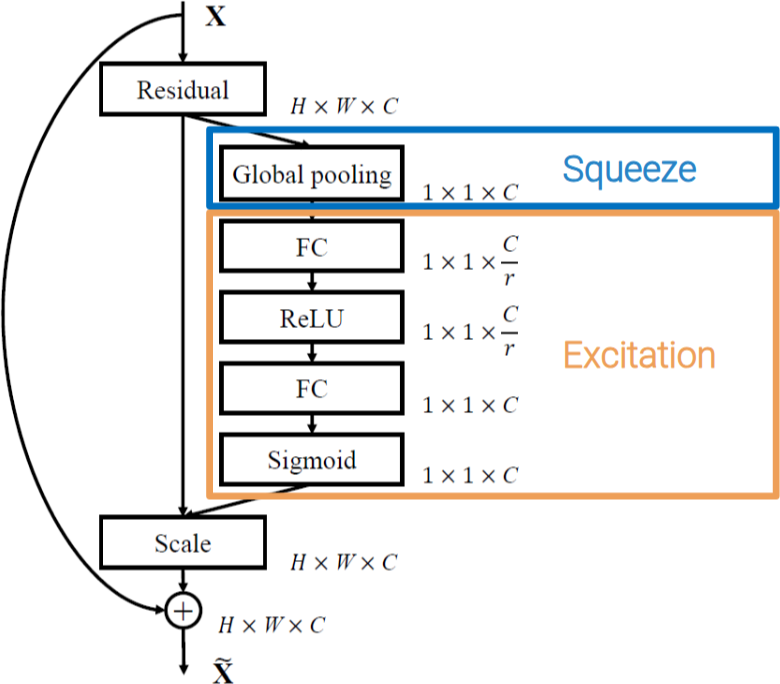
\includegraphics[width=0.4\linewidth]{./img/se_resnet.png}
            \caption{SE-ResNet module}
        \end{figure}
\end{description}



\section{MobileNetV2}

\begin{description}
    \item[Depth-wise separable convolution] \marginnote{Depth-wise separable convolution} 
        Use grouped convolutions to reduce the computational cost of standard convolutions. The operations of filtering and combining features are split:
        \begin{descriptionlist}
            \item[Depth-wise convolution]
                Processes each channel in isolation. In other words, a grouped convolution with groups equal to the number of input channels is applied.

            \item[Context point-wise convolution]
                $1 \times 1$ convolution applied after the depth-wise convolution to reproduce the channel-wide effect of standard convolutions.
        \end{descriptionlist}

        \begin{remark}
            The gain in computation is up to 10 times the FLOPs of normal convolutions.
        \end{remark}

        \begin{remark}
            Depth-wise convolutions are less expressive than normal convolutions.
        \end{remark}

        \begin{figure}[H]
            \centering
            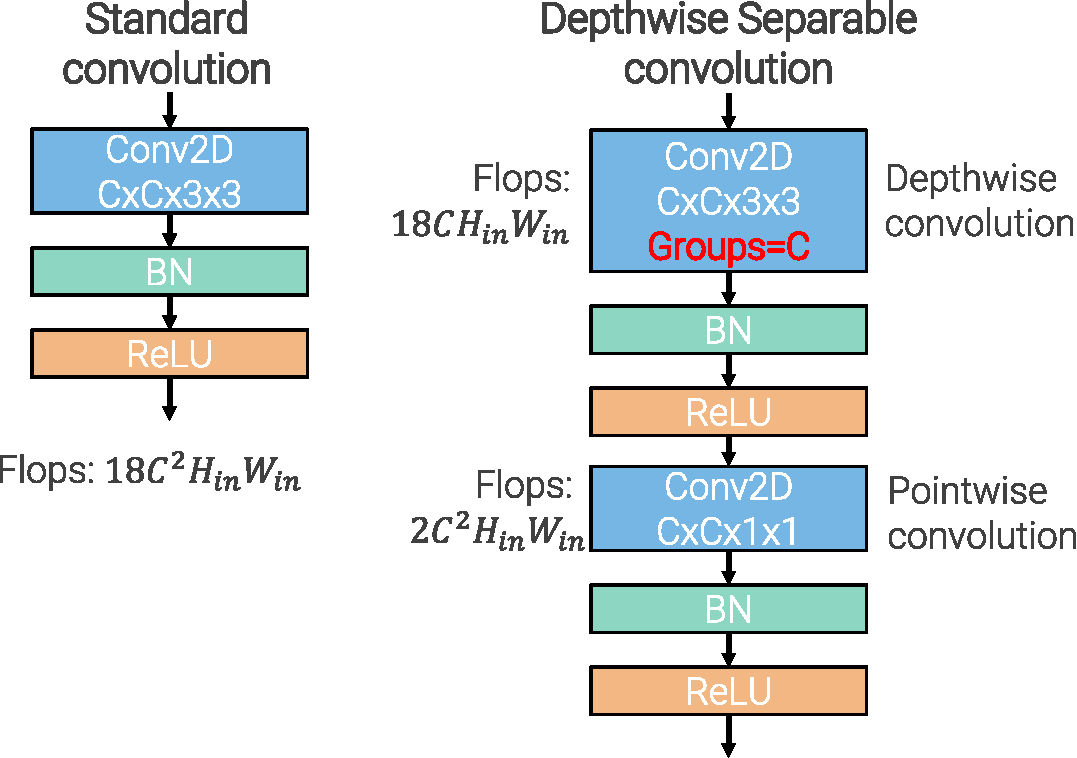
\includegraphics[width=0.45\linewidth]{./img/_depthwise_conv.pdf}
        \end{figure}
\end{description}

\begin{remark}
    The $3 \times 3$ convolution in bottleneck residual blocks process a compressed version of the input activation, which might cause loss of information when passing through the ReLUs.
\end{remark}

\begin{description}
    \item[Inverted residual block] \marginnote{Inverted residual block}
        Modified bottleneck block defined as follows:
        \begin{enumerate}
            \item A $1 \times 1$ convolution to expand the input channels by a factor of $t$. 
            \item A $3 \times 3$ depth-wise convolution.
            \item A $1 \times 1$ convolution to compress the channels back to the original shape.
        \end{enumerate}
        Moreover, non-linearity between residual blocks is removed as a result of theoretical studies.

        \begin{figure}[H]
            \centering
            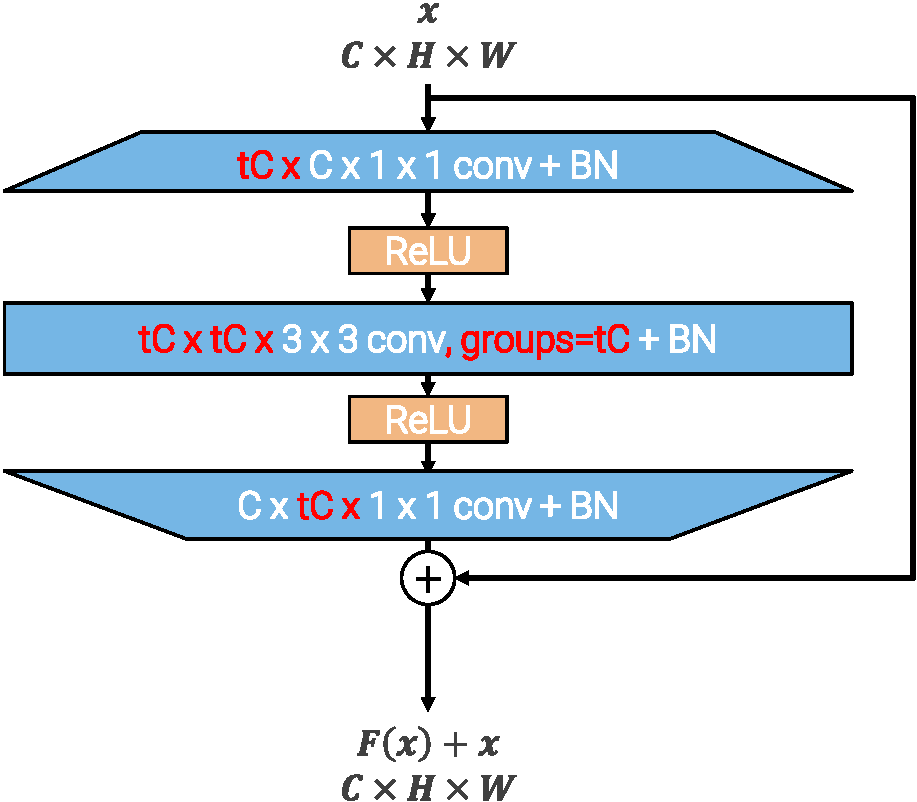
\includegraphics[width=0.4\linewidth]{./img/_inverted_residual.pdf}
        \end{figure}
\end{description}

\begin{description}
    \item[MobileNetV2] \marginnote{MobileNetV2} 
        Stack of inverted residual blocks.
        \begin{itemize}
            \item The number of channels grows slower compared to other architectures.
            \item The stem layer is lightweight due to the low number of intermediate channels.
            \item Due to the small number of channels, the number of channels in the activation are expanded before passing to the fully-connected layers.
        \end{itemize}

        \begin{remark}
            Stride $2$ is applied to the middle $3 \times 3$ convolution when downsampling is needed.
        \end{remark}

        \begin{table}[H]
            \centering
            \caption{\parbox[t]{0.6\linewidth}{Architecture of MobileNetV2 with expansion factor ($t$), number of channels ($c$), number of times a block is repeated ($n$), and stride ($s$).}}
            \small
            \begin{tabular}{cccccc}
                \toprule
                \textbf{Input}                       & \textbf{Operator}                      & $t$ & $c$     & $n$ & $s$ \\
                \midrule
                $2242 \times 3$             & \texttt{conv2d}               & - & 32    & 1 & 2 \\
                \midrule
                $1122 \times 32$            & \texttt{bottleneck}           & 1 & 16    & 1 & 1 \\
                $1122 \times 16$            & \texttt{bottleneck}           & 6 & 24    & 2 & 2 \\
                $562 \times 24$             & \texttt{bottleneck}           & 6 & 32    & 3 & 2 \\
                $282 \times 32$             & \texttt{bottleneck}           & 6 & 64    & 4 & 2 \\
                $142 \times 64$             & \texttt{bottleneck}           & 6 & 96    & 3 & 1 \\
                $142 \times 96$             & \texttt{bottleneck}           & 6 & 160   & 3 & 2 \\
                $72 \times 160$             & \texttt{bottleneck}           & 6 & 320   & 1 & 1 \\
                \midrule
                $72 \times 320$             & \texttt{conv2d $1\times1$}    & - & 1280  & 1 & 1 \\
                \midrule
                $72 \times 1280$            & \texttt{avgpool $7\times7$}   & - & -     & 1 & - \\
                $1 \times 1 \times 1280$    & \texttt{conv2d $1\times1$}    & - & k     & - & 1 \\
                \bottomrule
            \end{tabular}
        \end{table}
\end{description}



\section{Model scaling}

\begin{description}
    \item[Single dimension scaling]
        Scaling a baseline model by width, depth, or resolution. It generally always improve the accuracy.

        \begin{description}
            \item[Width scaling] \marginnote{Width scaling}
                Increase the number of channels.
            \item[Depth scaling] \marginnote{Depth scaling}
                Increase the number of blocks.
            \item[Resolution scaling] \marginnote{Resolution scaling}
                Increase the spatial dimension of the activations. 
        \end{description}

        \begin{figure}[H]
            \centering
            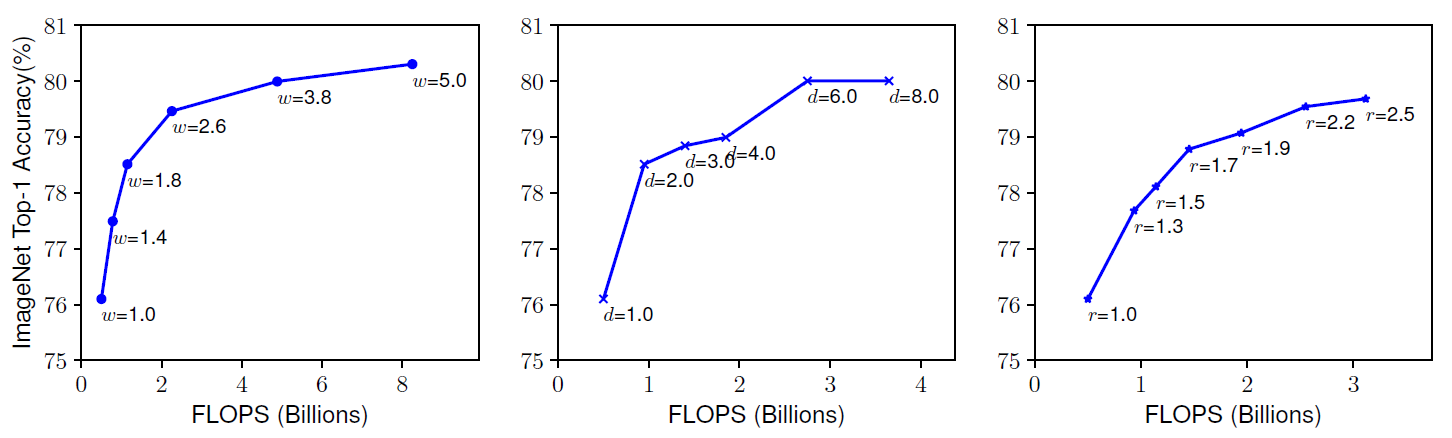
\includegraphics[width=0.85\linewidth]{./img/single_model_scaling.png}
            \caption{\parbox[t]{0.7\linewidth}{Top-1 accuracy variation with width, depth, and resolution scaling on EfficientNet}}
        \end{figure}

    \item[Compound scaling] \marginnote{Compound scaling}
        Scaling across multiple dimensions.

        \begin{figure}[H]
            \centering
            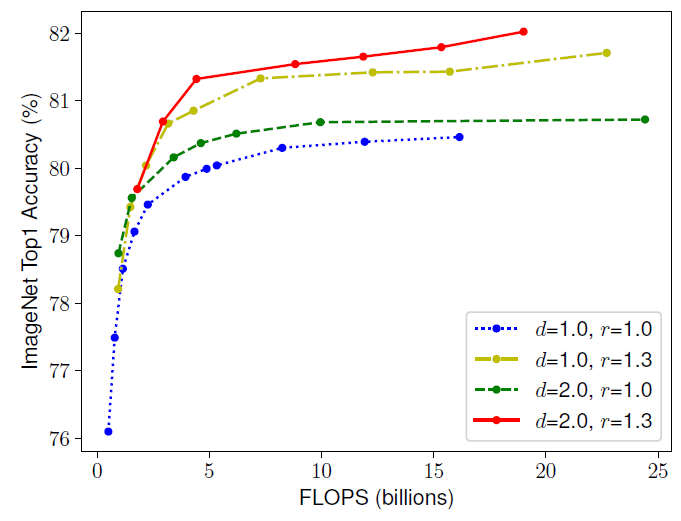
\includegraphics[width=0.45\linewidth]{./img/compound_scaling.png}
            \caption{Width scaling for different fixed depths and resolutions}
        \end{figure}

        \begin{description}
            \item[Compound scaling coefficient]
                Use a compound coefficient $\phi$ to scale dimensions and systematically control the FLOPs increase.
                \begin{remark}
                    $\phi=0$ represents the baseline model.
                \end{remark}

                The multiplier for depth ($d$), width ($w$), and resolution ($r$) are determined as:
                \[ d = \alpha^\phi \qquad w = \beta^\phi \qquad r = \gamma^\phi \]
                where $\alpha$, $\beta$, and $\gamma$ are subject to:
                \[ \alpha \cdot \beta^2 \cdot \gamma^2 \approx 2 \qquad \text{with } \alpha, \beta, \gamma \geq 1 \]
                By enforcing this constraint, FLOPs will approximately grow by $2^\phi$ (i.e., double) for each increase of $\phi$. 

                In practice, $\alpha$, $\beta$, and $\gamma$ are determined through grid search.

                \begin{remark}
                    The constraint is formulated in this way as FLOPS scales linearly with depth but quadratically with width and resolution.
                \end{remark}
        \end{description}
\end{description}

\begin{figure}[H]
    \centering
    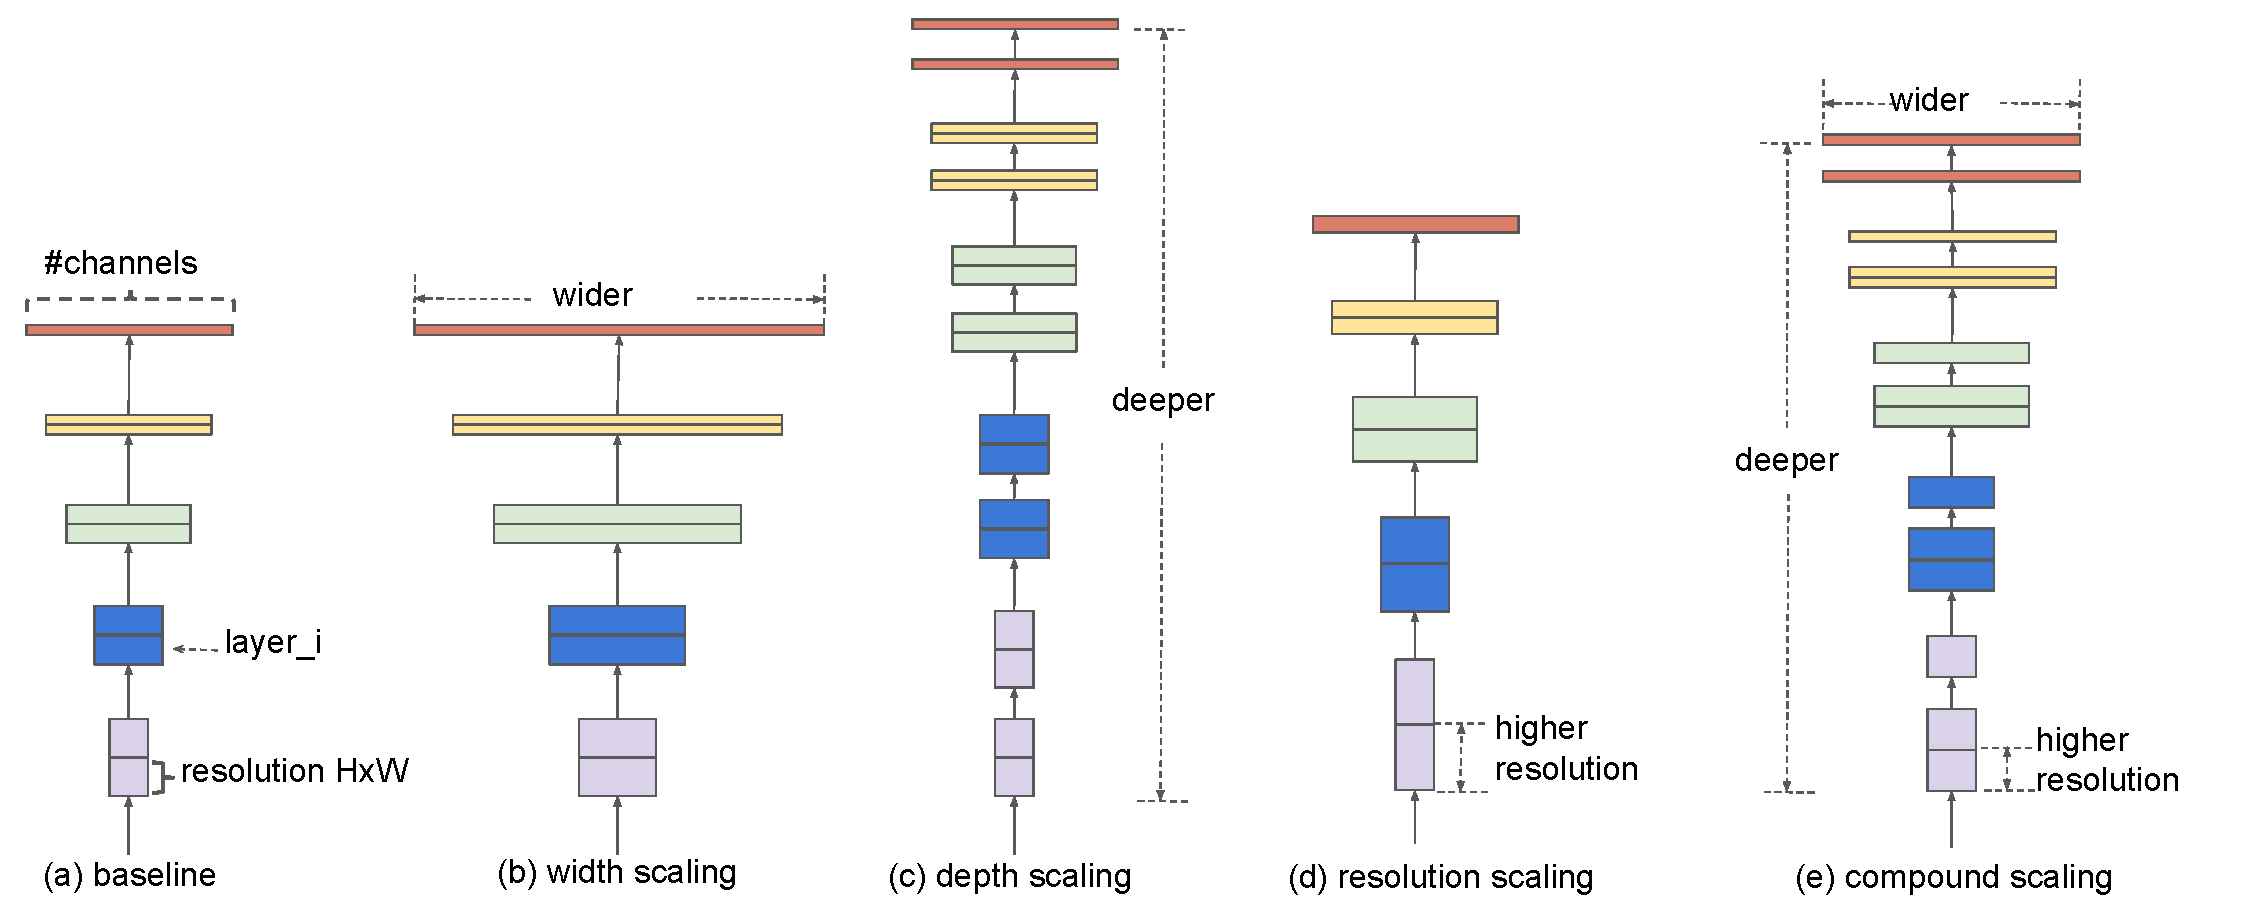
\includegraphics[width=0.95\linewidth]{./img/_model_scaling.pdf}
    \caption{Model scaling approaches}
\end{figure}


\subsection{Wide ResNet}

\begin{description}
    \item[Wide ResNet (WRN)] \marginnote{Wide ResNet (WRN)}
        ResNet scaled width-wise.

        \begin{figure}[H]
            \centering
            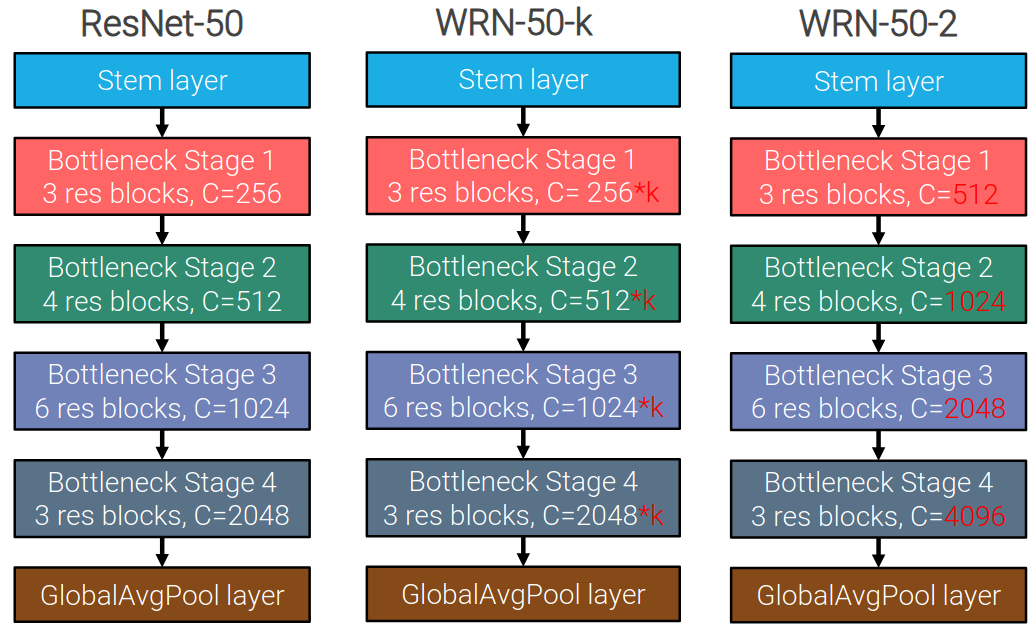
\includegraphics[width=0.5\linewidth]{./img/wide_resnet.png}
        \end{figure}

        \begin{remark}
            Wider layers are easier to parallelize on GPUs.
        \end{remark}
\end{description}



\section{EfficientNet}

\begin{description}
    \item[Neural architecture search (NAS)] \marginnote{Neural architecture search (NAS)}
        Train a controller neural network using gradient policy to output network architectures.

        \begin{figure}[H]
            \centering
            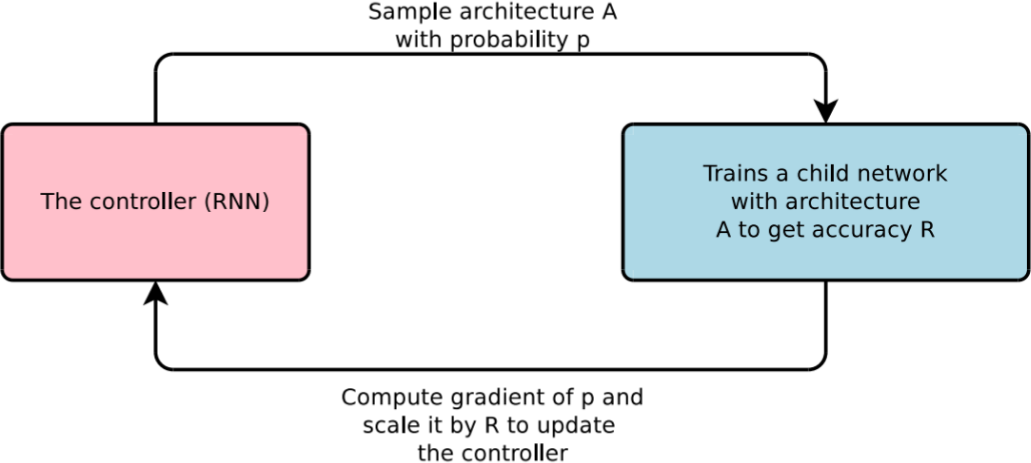
\includegraphics[width=0.45\linewidth]{./img/neural_architecture_search.png}
        \end{figure}

        \begin{remark}
            Although effective, we usually cannot extract guiding principles from the architecture outputted by NAS.
        \end{remark}

    \item[EfficientNet-B0] \marginnote{EfficientNet-B0}
        Architecture obtained through neural architecture search starting from MobileNet.

        Scaling the baseline model (B0) allowed obtaining high accuracies with a controlled number of FLOPs.
        \begin{figure}[H]
            \centering
            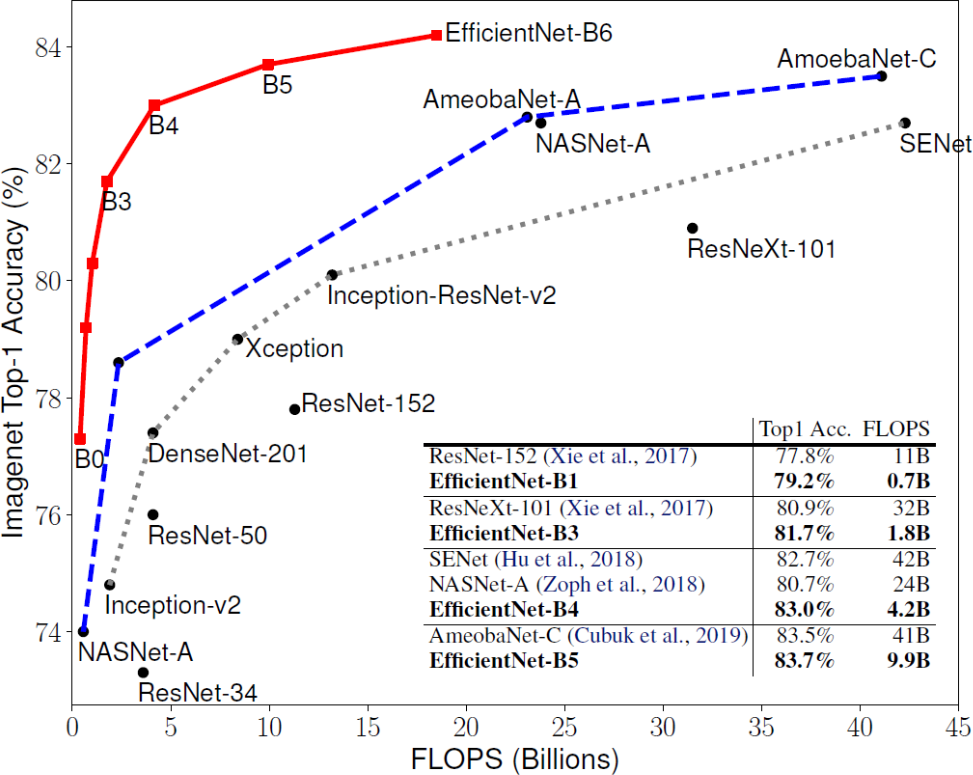
\includegraphics[width=0.45\linewidth]{./img/efficientnet_scaling.png}
        \end{figure}
\end{description}



\section{RegNet}

\begin{description}
    \item[Design space] \marginnote{Design space}
        Space of a parametrized population of neural network architectures. By sampling networks from a design space, it is possible to determine a distribution and evaluate it using statistical tools.

        \begin{remark}
            Comparing distributions is more robust than searching for a single well performing architecture (as in NAS).
        \end{remark}
    
    \item[RegNet] \marginnote{RegNet}
        Classic stem-body-head architecture (similar to ResNeXt with fewer constraints) with four stages. Each stage $i$ has the following parameters:
        \begin{itemize}
            \item Number of blocks (i.e., depth) $d_i$.
            \item Width of the blocks $w_i$ (so each stage does not necessarily double the number of channels).
            \item Number of groups of each block $g_i$.
            \item Bottleneck ratio of each block $b_i$.
        \end{itemize}

        \begin{figure}[H]
            \centering
            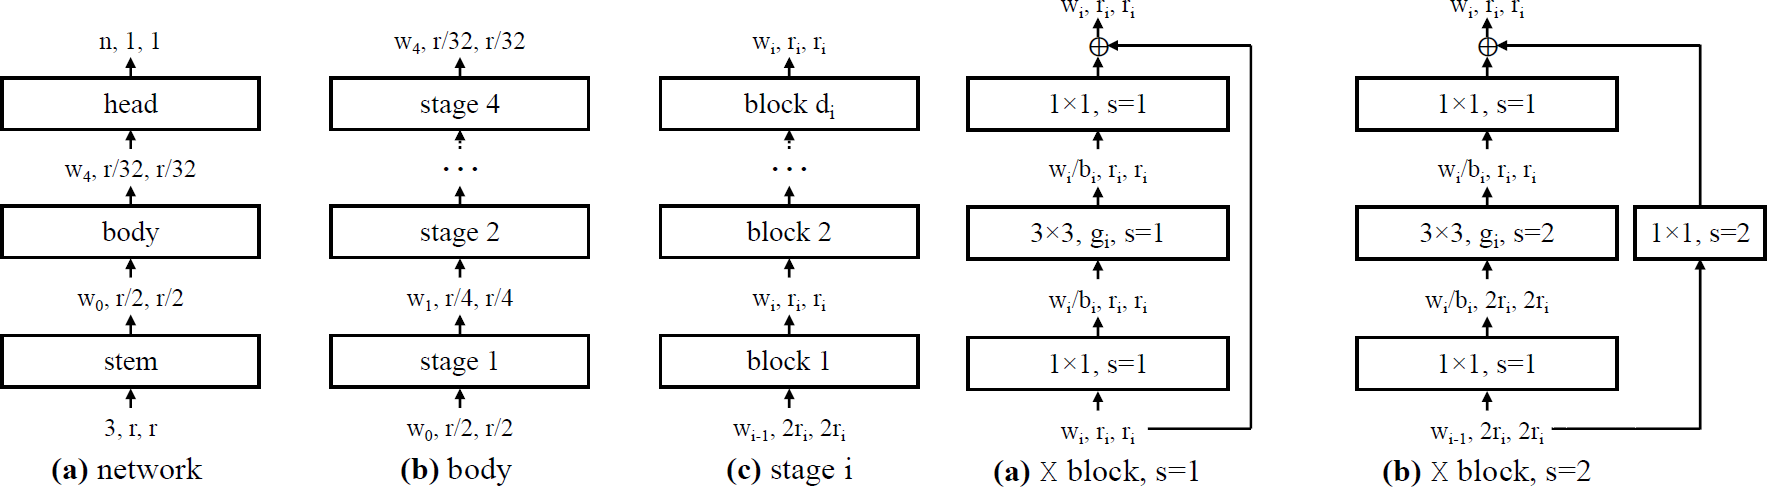
\includegraphics[width=0.95\linewidth]{./img/regnet.png}
        \end{figure}

        In other words, RegNet defines a $16$-dimensional design space. To evaluate the architectures, the following is done:
        \begin{enumerate}
            \item Sample $n=500$ models from the design space and train them on a low-epoch training regime.
            \item Determine the error empirical cumulative distribution function $F$ computed as the fraction of models with an error less than $e$:
            \[ F(e) = \frac{1}{n} \sum_{i=1}^{n} \mathbf{1}[e_i < e] \]
            \item Evaluate the design space by plotting $F$.
                \begin{figure}[H]
                    \centering
                    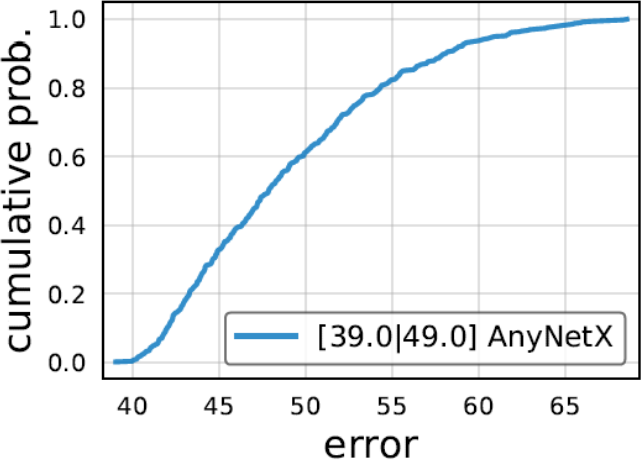
\includegraphics[width=0.25\linewidth]{./img/edf.png}
                    \caption{Example of cumulative distribution}
                \end{figure}

                \begin{remark}
                    Similarly to the ROC curve, the plot of the perfect design space is a straight line at $1.0$ probability starting from $0\%$ error rate.
                \end{remark}
            \item Repeat by fixing or finding relationships between parameters (i.e., try to reduce the search space).
        \end{enumerate}
\end{description}

\begin{remark}
    In the original paper, RegNet outperformed EfficientNet. However, results were computed by retraining EfficientNet using the same hyperparameter configuration of RegNet, while the original paper of EfficientNet explicitly tuned its hyperparameters to maximize the results.
\end{remark}